% !TEX root = ../../ctfp-print.tex

\lettrine[lhang=0.17]{S}{o far} I've been glossing over the meaning of function types. A function
type is different from other types.

Take \code{Integer}, for instance: It's just a set of integers.
\code{Bool} is a two element set. But a function type
$a\to b$ is more than that: it's a set of morphisms
between objects $a$ and $b$. A set of morphisms between
two objects in any category is called a hom-set. It just so happens that
in the category $\Set$ every hom-set is itself an object in the
same category ---because it is, after all, a \emph{set}.

\begin{figure}[H]
\centering
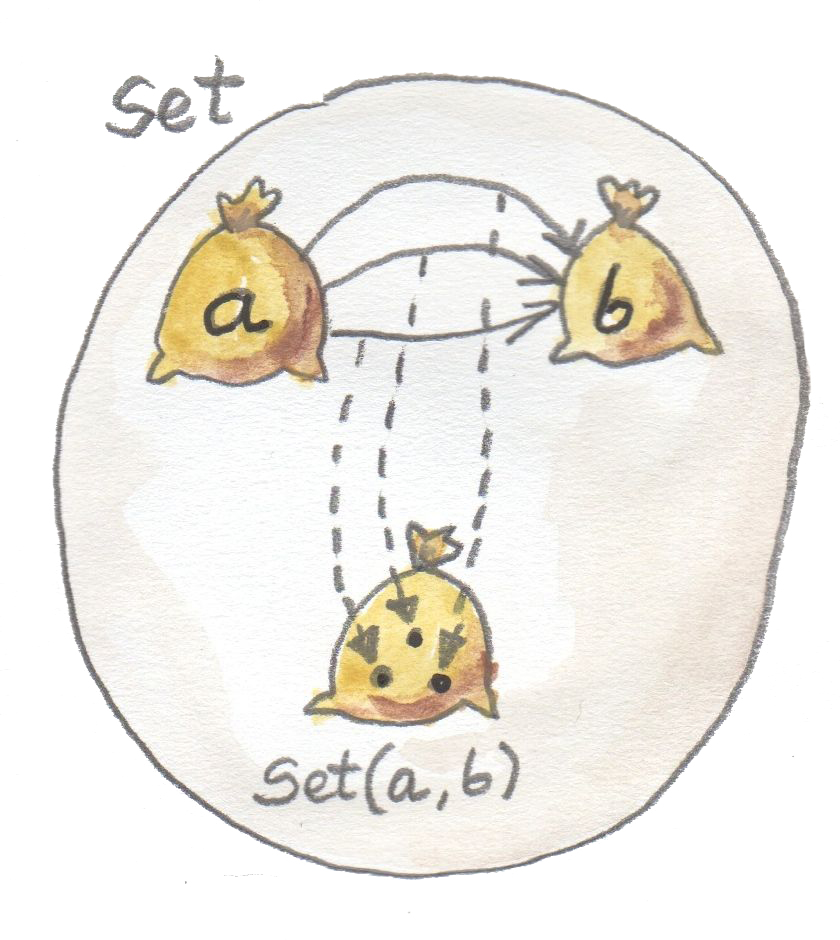
\includegraphics[width=0.35\textwidth]{images/set-hom-set.jpg}
\caption{Hom-set in Set is just a set}
\end{figure}

\noindent
The same is not true of other categories where hom-sets are external to
a category. They are even called \emph{external} hom-sets.

\begin{figure}[H]
\centering
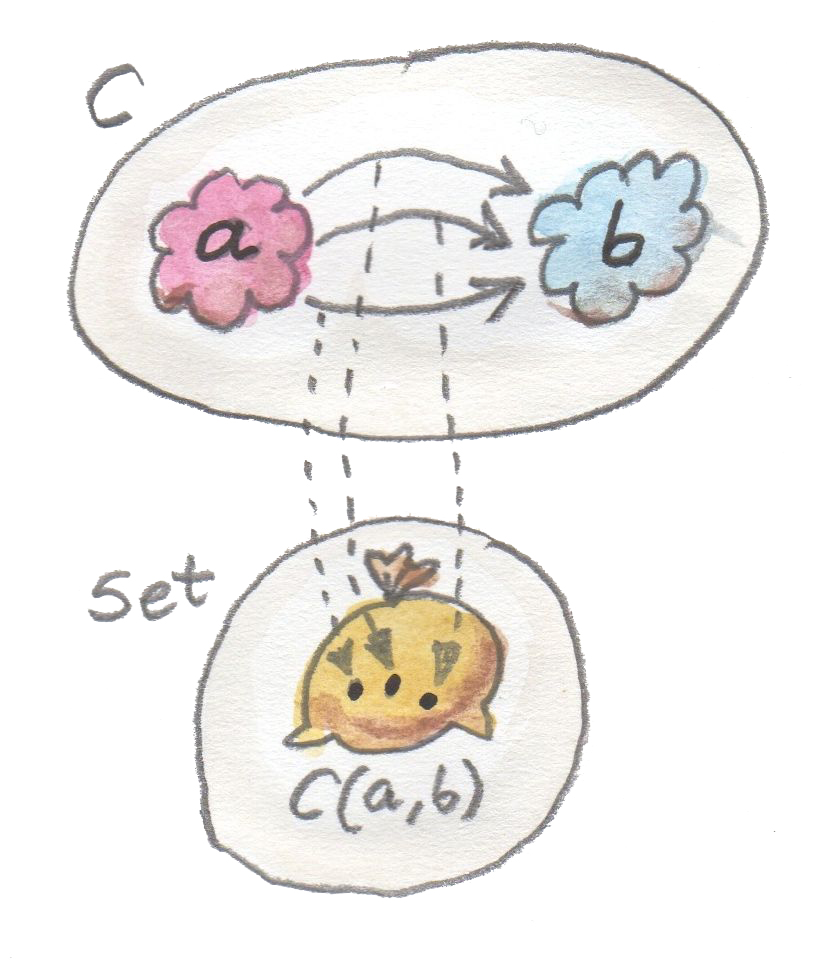
\includegraphics[width=0.35\textwidth]{images/hom-set.jpg}
\caption{Hom-set in category C is an external set}
\end{figure}

\noindent
It's the self-referential nature of the category $\Set$ that makes
function types special. But there is a way, at least in some categories,
to construct objects that represent hom-sets. Such objects are called
\newterm{internal} hom-sets.

\section{Universal Construction}

Let's forget for a moment that function types are sets and try to
construct a function type, or more generally, an internal hom-set, from
scratch. As usual, we'll take our cues from the $\Set$ category,
but carefully avoid using any properties of sets, so that the
construction will automatically work for other categories.

A function type may be considered a composite type because of its
relationship to the argument type and the result type. We've already
seen the constructions of composite types --- those that involved
relationships between objects. We used universal constructions to define
a \hyperref[products-and-coproducts]{product
and coproduct types}. We can use the same trick to define a
function type. We will need a pattern that involves three objects: the
function type that we are constructing, the argument type, and the
result type.

The obvious pattern that connects these three types is called
\newterm{function application} or \newterm{evaluation}. Given a candidate for
a function type, let's call it $z$ (notice that, if we are not in
the category $\Set$, this is just an object like any other
object), and the argument type $a$ (an object), the application
maps this pair to the result type $b$ (an object). We have three
objects, two of them fixed (the ones representing the argument type and
the result type).

We also have the application, which is a mapping. How do we incorporate
this mapping into our pattern? If we were allowed to look inside
objects, we could pair a function $f$ (an element of $z$)
with an argument $x$ (an element of $a$) and map it to
$f x$ (the application of $f$ to $x$, which is an
element of $b$).

\begin{figure}[H]
\centering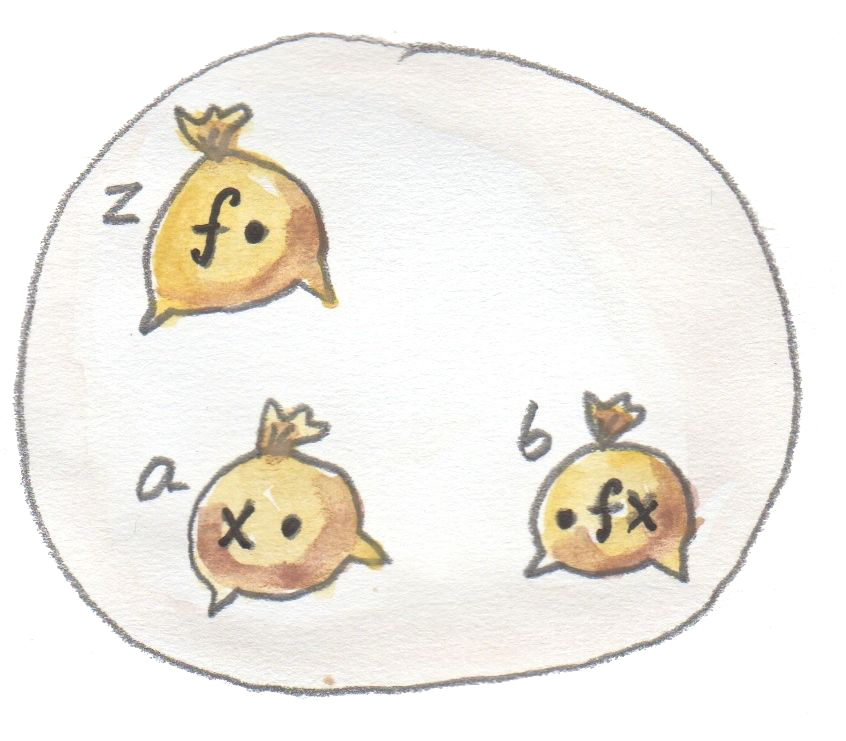
\includegraphics[width=0.35\textwidth]{images/functionset.jpg}
\caption{In Set we can pick a function $f$ from a set of functions $z$ and we can
pick an argument $x$ from the set (type) $a$. We get an element $f x$ in the
set (type) $b$.}
\end{figure}

\noindent
But instead of dealing with individual pairs $(f, x)$, we can as
well talk about the whole \emph{product} of the function type $z$
and the argument type $a$. The product $z\times{}a$ is an object,
and we can pick, as our application morphism, an arrow $g$ from
that object to $b$. In $\Set$, $g$ would be the
function that maps every pair $(f, x)$ to $f x$.

So that's the pattern: a product of two objects $z$ and
$a$ connected to another object $b$ by a morphism $g$.

\begin{figure}[H]
\centering
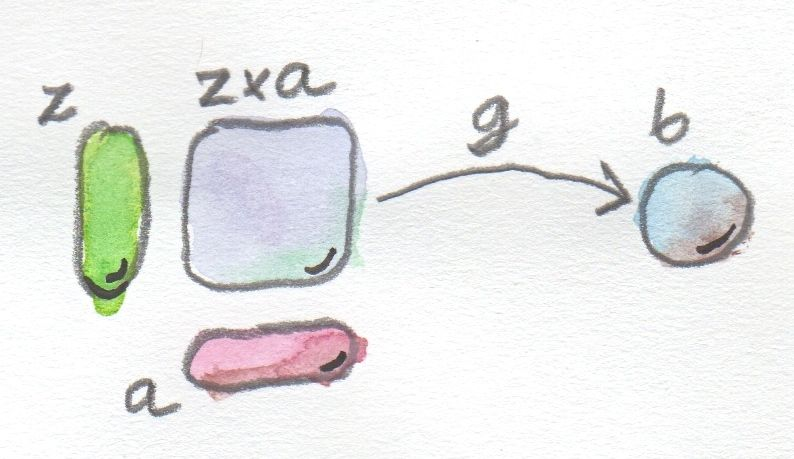
\includegraphics[width=0.4\textwidth]{images/functionpattern.jpg}
\caption{A pattern of objects and morphisms that is the starting point of the
universal construction}
\end{figure}

\noindent
Is this pattern specific enough to single out the function type using a
universal construction? Not in every category. But in the categories of
interest to us it is. And another question: Would it be possible to
define a function object without first defining a product? There are
categories in which there is no product, or there isn't a product for
all pairs of objects. The answer is no: there is no function type, if
there is no product type. We'll come back to this later when we talk
about exponentials.

Let's review the universal construction. We start with a pattern of
objects and morphisms. That's our imprecise query, and it usually yields
lots and lots of hits. In particular, in $\Set$, pretty much
everything is connected to everything. We can take any object
$z$, form its product with $a$, and there's going to be a
function from it to $b$ (except when $b$ is an empty set).

That's when we apply our secret weapon: ranking. This is usually done by
requiring that there be a unique mapping between candidate objects --- a
mapping that somehow factorizes our construction. In our case, we'll
decree that $z$ together with the morphism $g$ from
$z \times a$ to $b$ is \emph{better} than some other
$z'$ with its own application $g'$, if and
only if there is a unique mapping $h$ from $z'$ to
$z$ such that the application of $g'$ factors
through the application of $g$. (Hint: Read this sentence while
looking at the picture.)

\begin{figure}[H]
\centering
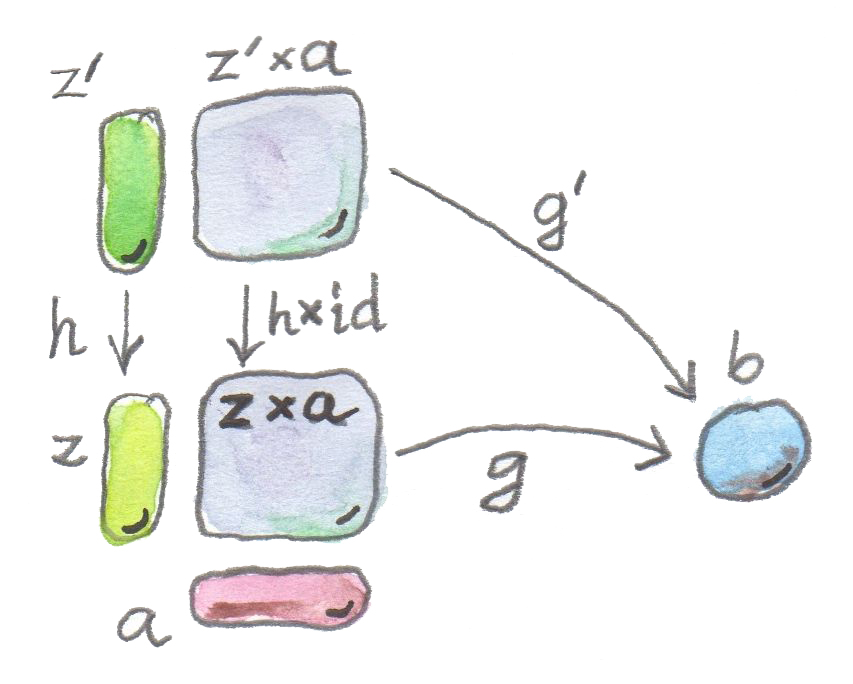
\includegraphics[width=0.4\textwidth]{images/functionranking.jpg}
\caption{Establishing a ranking between candidates for the function object}
\end{figure}

\noindent
Now here's the tricky part, and the main reason I postponed this
particular universal construction till now. Given the morphism
$h \Colon z'\to z$, we want to close the diagram
that has both $z'$ and $z$ crossed with $a$.
What we really need, given the mapping $h$ from $z'$
to $z$, is a mapping from $z' \times a$ to $z \times a$.
And now, after discussing the \hyperref[functoriality]{functoriality
of the product}, we know how to do it. Because the product itself is a
functor (more precisely an endo-bi-functor), it's possible to lift pairs
of morphisms. In other words, we can define not only products of objects
but also products of morphisms.

Since we are not touching the second component of the product
$z' \times a$, we will lift the pair of morphisms
$(h, \id)$, where $\id$ is an identity on $a$.

So, here's how we can factor one application, $g$, out of another
application $g'$:
\[g' = g \circ (h \times \id)\]
The key here is the action of the product on morphisms.

The third part of the universal construction is selecting the object
that is universally the best. Let's call this object $a \Rightarrow b$ (think
of this as a symbolic name for one object, not to be confused with a
Haskell typeclass constraint --- I'll discuss different ways of naming
it later). This object comes with its own application --- a morphism
from $(a \Rightarrow b) \times a$ to $b$ --- which we will call
$eval$. The object \code{$a \Rightarrow b$} is the best if any other
candidate for a function object can be uniquely mapped to it in such a
way that its application morphism $g$ factorizes through
$eval$. This object is better than any other object according to
our ranking.

\begin{figure}[H]
\centering
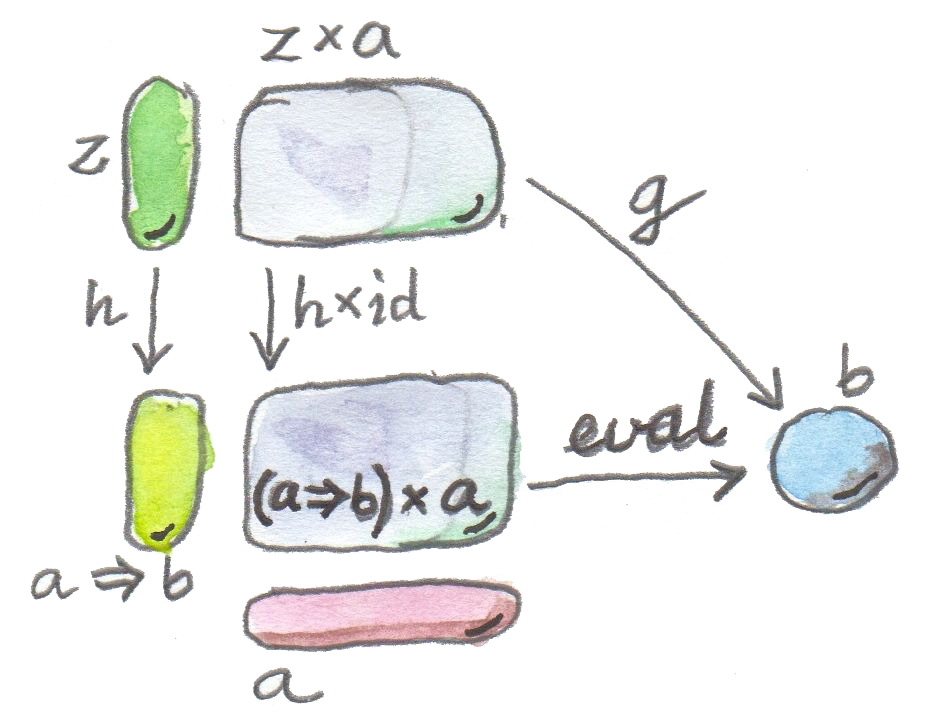
\includegraphics[width=0.4\textwidth]{images/universalfunctionobject.jpg}
\caption{The definition of the universal function object. This is the same
diagram as above, but now the object $a \Rightarrow b$ is \emph{universal}.}
\end{figure}

\noindent
Formally:

\begin{longtable}[]{@{}l@{}}
\toprule
\begin{minipage}[t]{0.97\columnwidth}\raggedright\strut
A \emph{function object} from $a$ to $b$ is an object
$a \Rightarrow b$ together with the morphism
\[eval \Colon ((a \Rightarrow b) \times a) \to b\]
such that for any other object $z$ with a morphism
\[g \Colon z \times a \to b\]
there is a unique morphism
\[h \Colon z \to (a \Rightarrow b)\]
that factors $g$ through $eval$:
\[g = eval \circ (h \times \id)\]
\end{minipage}\tabularnewline
\bottomrule
\end{longtable}

\noindent
Of course, there is no guarantee that such an object $a \Rightarrow b$ exists
for any pair of objects $a$ and $b$ in a given category.
But it always does in $\Set$. Moreover, in $\Set$, this
object is isomorphic to the hom-set $\Set(a, b)$.

This is why, in Haskell, we interpret the function type
\code{a -> b} as the categorical function object $a \Rightarrow b$.

\section{Currying}

Let's have a second look at all the candidates for the function object.
This time, however, let's think of the morphism $g$ as a function
of two variables, $z$ and $a$.
\[g \Colon z \times a \to b\]
Being a morphism from a product comes as close as it gets to being a
function of two variables. In particular, in $\Set$, $g$ is
a function from pairs of values, one from the set $z$ and one
from the set $a$.

On the other hand, the universal property tells us that for each such
$g$ there is a unique morphism $h$ that maps $z$ to
a function object $a \Rightarrow b$.
\[h \Colon z \to (a \Rightarrow b)\]
In $\Set$, this just means that $h$ is a function that
takes one variable of type $z$ and returns a function from
$a$ to $b$. That makes $h$ a higher order function.
Therefore the universal construction establishes a one-to-one
correspondence between functions of two variables and functions of one
variable returning functions. This correspondence is called
\newterm{currying}, and $h$ is called the curried version of $g$.

This correspondence is one-to-one, because given any $g$ there is
a unique $h$, and given any $h$ you can always recreate
the two-argument function $g$ using the formula:
\[g = eval \circ (h \times \id)\]
The function $g$ can be called the \emph{uncurried} version of $h$.

Currying is essentially built into the syntax of Haskell. A function
returning a function:

\src{snippet01}
is often thought of as a function of two variables. That's how we read
the un-parenthesized signature:

\src{snippet02}
This interpretation is apparent in the way we define multi-argument
functions. For instance:

\src{snippet03}
The same function can be written as a one-argument function returning a
function --- a lambda:

\src{snippet04}
These two definitions are equivalent, and either can be partially
applied to just one argument, producing a one-argument function, as in:

\src{snippet05}
Strictly speaking, a function of two variables is one that takes a pair
(a product type):

\src{snippet06}
It's trivial to convert between the two representations, and the two
(higher-order) functions that do it are called, unsurprisingly,
\code{curry} and \code{uncurry}:

\src{snippet07}
and

\src{snippet08}
Notice that \code{curry} is the \emph{factorizer} for the universal
construction of the function object. This is especially apparent if it's
rewritten in this form:

\src{snippet09}
(As a reminder: A factorizer produces the factorizing function from a
candidate.)

In non-functional languages, like C++, currying is possible but
nontrivial. You can think of multi-argument functions in C++ as
corresponding to Haskell functions taking tuples (although, to confuse
things even more, in C++ you can define functions that take an explicit
\code{std::tuple}, as well as variadic functions, and functions taking
initializer lists).

You can partially apply a C++ function using the template
\code{std::bind}. For instance, given a function of two strings:

\begin{snip}{cpp}
std::string catstr(std::string s1, std::string s2) {
    return s1 + s2;
}
\end{snip}
you can define a function of one string:

\begin{snip}{cpp}
using namespace std::placeholders;

auto greet = std::bind(catstr, "Hello ", _1);
std::cout << greet("Haskell Curry");
\end{snip}
Scala, which is more functional than C++ or Java, falls somewhere in
between. If you anticipate that the function you're defining will be
partially applied, you define it with multiple argument lists:

\begin{snip}{cpp}
def catstr(s1: String)(s2: String) = s1 + s2
\end{snip}
Of course that requires some amount of foresight or prescience on the
part of a library writer.

\section{Exponentials}

In mathematical literature, the function object, or the internal
hom-object between two objects $a$ and $b$, is often
called the \newterm{exponential} and denoted by $b^{a}$. Notice that
the argument type is in the exponent. This notation might seem strange
at first, but it makes perfect sense if you think of the relationship
between functions and products. We've already seen that we have to use
the product in the universal construction of the internal hom-object,
but the connection goes deeper than that.

This is best seen when you consider functions between finite types ---
types that have a finite number of values, like \code{Bool},
\code{Char}, or even \code{Int} or \code{Double}. Such functions,
at least in principle, can be fully memoized or turned into data
structures to be looked up. And this is the essence of the equivalence
between functions, which are morphisms, and function types, which are
objects.

For instance a (pure) function from \code{Bool} is completely
specified by a pair of values: one corresponding to \code{False}, and
one corresponding to \code{True}. The set of all possible functions
from \code{Bool} to, say, \code{Int} is the set of all pairs of
\code{Int}s. This is the same as the product \code{Int} × \code{Int} or,
being a little creative with notation, \code{Int}\textsuperscript{2}.

For another example, let's look at the C++ type \code{char}, which
contains 256 values (Haskell \code{Char} is larger, because Haskell
uses Unicode). There are several functions in the part of the
C++ Standard Library that are usually implemented using lookups.
Functions like \code{isupper} or \code{isspace} are implemented
using tables, which are equivalent to tuples of 256 Boolean values. A
tuple is a product type, so we are dealing with products of 256
Booleans: \code{bool × bool × bool × ... × bool}. We know from
arithmetics that an iterated product defines a power. If you
``multiply'' \code{bool} by itself 256 (or \code{char}) times, you
get \code{bool} to the power of \code{char}, or \code{bool}\textsuperscript{\code{char}}.

How many values are there in the type defined as 256-tuples of
\code{bool}? Exactly $2^{256}$. This is also the number
of different functions from \code{char} to \code{bool}, each
function corresponding to a unique 256-tuple. You can similarly
calculate that the number of functions from \code{bool} to
\code{char} is $256^{2}$, and so on. The exponential
notation for function types makes perfect sense in these cases.

We probably wouldn't want to fully memoize a function from \code{int}
or \code{double}. But the equivalence between functions and data
types, if not always practical, is there. There are also infinite types,
for instance lists, strings, or trees. Eager memoization of functions
from those types would require infinite storage. But Haskell is a lazy
language, so the boundary between lazily evaluated (infinite) data
structures and functions is fuzzy. This function vs. data duality
explains the identification of Haskell's function type with the
categorical exponential object --- which corresponds more to our idea of
\emph{data}.

\section{Cartesian Closed Categories}

Although I will continue using the category of sets as a model for types
and functions, it's worth mentioning that there is a larger family of
categories that can be used for that purpose. These categories are
called \newterm{Cartesian closed}, and $\Set$ is just one example of
such a category.

A Cartesian closed category must contain:

\begin{enumerate}
\tightlist
\item
  The terminal object,
\item
  A product of any pair of objects, and
\item
  An exponential for any pair of objects.
\end{enumerate}
If you consider an exponential as an iterated product (possibly
infinitely many times), then you can think of a Cartesian closed
category as one supporting products of an arbitrary arity. In
particular, the terminal object can be thought of as a product of zero
objects --- or the zero-th power of an object.

What's interesting about Cartesian closed categories from the
perspective of computer science is that they provide models for the
simply typed lambda calculus, which forms the basis of all typed
programming languages.

The terminal object and the product have their duals: the initial object
and the coproduct. A Cartesian closed category that also supports those
two, and in which product can be distributed over coproduct
\begin{gather*}
a \times (b + c) = a \times b + a \times c \\
(b + c) \times a = b \times a + c \times a
\end{gather*}
is called a \newterm{bicartesian closed} category. We'll see in the next
section that bicartesian closed categories, of which $\Set$ is a
prime example, have some interesting properties.

\section{Exponentials and Algebraic Data Types}

The interpretation of function types as exponentials fits very well into
the scheme of algebraic data types. It turns out that all the basic
identities from high-school algebra relating numbers zero and one, sums,
products, and exponentials hold pretty much unchanged in any bicartesian
closed category for, respectively, initial and final objects,
coproducts, products, and exponentials. We don't have the tools yet to
prove them (such as adjunctions or the Yoneda lemma), but I'll list them
here nevertheless as a source of valuable intuitions.

\subsection{Zeroth Power}

\[a^{0} = 1\]
In the categorical interpretation, we replace 0 with the initial object,
1 with the final object, and equality with isomorphism. The exponential
is the internal hom-object. This particular exponential represents the
set of morphisms going from the initial object to an arbitrary object
$a$. By the definition of the initial object, there is exactly
one such morphism, so the hom-set $\cat{C}(0, a)$ is a singleton set. A
singleton set is the terminal object in $\Set$, so this identity
trivially works in $\Set$. What we are saying is that it works in
any bicartesian closed category.

In Haskell, we replace 0 with \code{Void}; 1 with the unit type
\code{()}; and the exponential with function type. The claim is that
the set of functions from \code{Void} to any type \code{a} is
equivalent to the unit type --- which is a singleton. In other words,
there is only one function \code{Void -> a}. We've seen
this function before: it's called \code{absurd}.

This is a little bit tricky, for two reasons. One is that in Haskell we
don't really have uninhabited types --- every type contains the ``result
of a never ending calculation,'' or the bottom. The second reason is
that all implementations of \code{absurd} are equivalent because, no
matter what they do, nobody can ever execute them. There is no value
that can be passed to \code{absurd}. (And if you manage to pass it a
never ending calculation, it will never return!)

\subsection{Powers of One}

\[1^{a} = 1\]
This identity, when interpreted in $\Set$, restates the definition
of the terminal object: There is a unique morphism from any object to
the terminal object. In general, the internal hom-object from $a$
to the terminal object is isomorphic to the terminal object itself.

In Haskell, there is only one function from any type \code{a} to unit.
We've seen this function before --- it's called \code{unit}. You can
also think of it as the function \code{const} partially applied to
\code{()}.

\subsection{First Power}

\[a^{1} = a\]
This is a restatement of the observation that morphisms from the
terminal object can be used to pick ``elements'' of the object
\code{a}. The set of such morphisms is isomorphic to the object
itself. In $\Set$, and in Haskell, the isomorphism is between
elements of the set \code{a} and functions that pick those elements,
\code{() -> a}.

\subsection{Exponentials of Sums}

\[a^{b+c} = a^{b} \times a^{c}\]
Categorically, this says that the exponential from a coproduct of two
objects is isomorphic to a product of two exponentials. In Haskell, this
algebraic identity has a very practical, interpretation. It tells us
that a function from a sum of two types is equivalent to a pair of
functions from individual types. This is just the case analysis that we
use when defining functions on sums. Instead of writing one function
definition with a \code{case} statement, we usually split it into two
(or more) functions dealing with each type constructor separately. For
instance, take a function from the sum type
\code{(Either Int Double)}:

\src{snippet10}
It may be defined as a pair of functions from, respectively,
\code{Int} and \code{Double}:

\src{snippet11}
Here, \code{n} is an \code{Int} and \code{x} is a \code{Double}.

\subsection{Exponentials of Exponentials}

\[(a^{b})^{c} = a^{b \times c}\]
This is just a way of expressing currying purely in terms of exponential
objects. A function returning a function is equivalent to a function
from a product (a two-argument function).

\subsection{Exponentials over Products}

\[(a \times b)^{c} = a^{c} \times b^{c}\]
In Haskell: A function returning a pair is equivalent to a pair of
functions, each producing one element of the pair.

It's pretty incredible how those simple high-school algebraic identities
can be lifted to category theory and have practical application in
functional programming.

\section{Curry-Howard Isomorphism}

I have already mentioned the correspondence between logic and algebraic
data types. The \code{Void} type and the unit type \code{()}
correspond to false and true. Product types and sum types correspond to
logical conjunction $\wedge$ (AND) and disjunction $\vee$ (OR). In this scheme, the
function type we have just defined corresponds to logical implication $\Rightarrow$.
In other words, the type \code{a -> b} can be read as ``if
a then b.''

According to the Curry-Howard isomorphism, every type can be interpreted
as a proposition --- a statement or a judgment that may be true or
false. Such a proposition is considered true if the type is inhabited
and false if it isn't. In particular, a logical implication is true if
the function type corresponding to it is inhabited, which means that
there exists a function of that type. An implementation of a function is
therefore a proof of a theorem. Writing programs is equivalent to
proving theorems. Let's see a few examples.

Let's take the function \code{eval} we have introduced in the
definition of the function object. Its signature is:

\src{snippet12}
It takes a pair consisting of a function and its argument and produces a
result of the appropriate type. It's the Haskell implementation of the
morphism:

\[eval \Colon (a \Rightarrow b) \times a \to b\]
which defines the function type $a \Rightarrow b$ (or the exponential object
$b^{a}$). Let's translate this signature to a logical predicate
using the Curry-Howard isomorphism:

\[((a \Rightarrow b) \wedge a) \Rightarrow b\]
Here's how you can read this statement: If it's true that $b$
follows from $a$, and $a$ is true, then $b$ must be
true. This makes perfect intuitive sense and has been known since
antiquity as \newterm{modus ponens}. We can prove this theorem by
implementing the function:

\src{snippet13}
If you give me a pair consisting of a function \code{f} taking
\code{a} and returning \code{b}, and a concrete value \code{x} of
type \code{a}, I can produce a concrete value of type \code{b} by
simply applying the function \code{f} to \code{x}. By implementing
this function I have just shown that the type
\code{((a -> b), a) -> b} is inhabited.
Therefore \newterm{modus ponens} is true in our logic.

How about a predicate that is blatantly false? For instance: if
$a$ or $b$ is true then $a$ must be true.

\[a \vee b \Rightarrow a\]
This is obviously wrong because you can choose an $a$ that is
false and a $b$ that is true, and that's a counter-example.

Mapping this predicate into a function signature using the Curry-Howard
isomorphism, we get:

\src{snippet14}
Try as you may, you can't implement this function --- you can't produce
a value of type \code{a} if you are called with the \code{Right}
value. (Remember, we are talking about \emph{pure} functions.)

Finally, we come to the meaning of the \code{absurd} function:

\src{snippet15}
Considering that \code{Void} translates into false, we get:

\[false \Rightarrow a\]
Anything follows from falsehood (\emph{ex falso quodlibet}). Here's one
possible proof (implementation) of this statement (function) in Haskell:

\begin{snip}{haskell}
absurd (Void a) = absurd a
\end{snip}
where \code{Void} is defined as:

\begin{snip}{haskell}
newtype Void = Void Void
\end{snip}
As always, the type \code{Void} is tricky. This definition makes it
impossible to construct a value because in order to construct one, you
would need to provide one. Therefore, the function \code{absurd} can
never be called.

These are all interesting examples, but is there a practical side to
Curry-Howard isomorphism? Probably not in everyday programming. But
there are programming languages like Agda or Coq, which take advantage
of the Curry-Howard isomorphism to prove theorems.

Computers are not only helping mathematicians do their work --- they are
revolutionizing the very foundations of mathematics. The latest hot
research topic in that area is called Homotopy Type Theory, and is an
outgrowth of type theory. It's full of Booleans, integers, products and
coproducts, function types, and so on. And, as if to dispel any doubts,
the theory is being formulated in Coq and Agda. Computers are
revolutionizing the world in more than one way.

\section{Bibliography}

\begin{enumerate}
\tightlist
\item
  Ralph Hinze, Daniel W. H. James,
  \urlref{http://www.cs.ox.ac.uk/ralf.hinze/publications/WGP10.pdf}{Reason
  Isomorphically!}. This paper contains proofs of all those high-school
  algebraic identities in category theory that I mentioned in this
  chapter.
\end{enumerate}
